\documentclass{beamer}

\setbeamertemplate{navigation symbols}{}
\setbeamertemplate{itemize items}[square]
\useoutertheme{shadow}
\setbeamertemplate{headline}{}

\mode<presentation>
{
\usepackage[utf8]{inputenc}
\usetheme{Warsaw}
\usepackage{bm}
\usepackage{amsmath}
\usepackage{ulem}
\usepackage{cancel}

} 
\usepackage{algorithm, algorithmic}
\usepackage{graphicx}
\usepackage{textcomp}
\usepackage[english]{babel}
\usepackage[utf8]{inputenc}
\usepackage[T1]{fontenc}

\title{Counting Number of Inversions in an Array}
\author {Harshdeep ~Singh\inst{1}  \and Jaya ~Ram\inst{2}  \and Shivansh Gupta\inst{3}}
\institute{
\inst{1} IIT2019105 \hspace{5pt}
\inst{2} IIT2019106 \hspace{5pt}
\inst{3} IIT2019107 \hspace{5pt}\\
(Batch 2, Group 3)
}
\date{19 March 2021}


\begin{document}

\begin{frame}
  \titlepage
\end{frame}

\begin{frame}
\frametitle{Outline}
\tableofcontents
\end{frame}

\section{Introduction}
\begin{frame}{\textbf{Introduction}}
\begin{itemize}
    \item The Inversion Count of an array \textbf{A} is the count of all the pairs $\bm{(i,j)}$ such that $\bm{i}<\bm{j}$ and $\bm{A[i]}>\bm{A[j]}$ \\
    
    \begin{figure}[htbp]
    \centerline{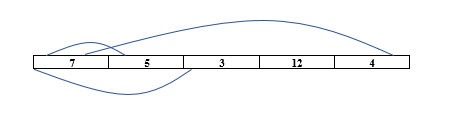
\includegraphics{inversion.png}}
    \caption{An example of inversion in array.}
    \label{fig}
    \end{figure}
    
    \item Thus, Inversion Count for an array indicates – how far the array is from being sorted.\\
\end{itemize}
\end{frame}

\section{Algorithm Description and Analysis}
\begin{frame}{\textbf{Algorithm Description and Analysis}}
\begin{block}{}
\textbf{Naive Approach}
involves a Brute Force approach where we iterate over all the pairs of the array (which can be done through a nested loop), and if any pair $(i,j)$ satisfies our condition, we increase our Inversion Count by one.
\end{block}

% \begin{block}{Divide and Conquer}
\textbf{Divide and Conquer Approach}\\
Suppose we divide our array A into two equal, or almost equal parts. Let's call the first one \textbf{L} and the other one \textbf{R}. Also, let's say we know the Inversion Count of both \textbf{L} and \textbf{R}. Let's call them $\bm{inv_1}$ and $\bm{inv_2}$. \\
Now, any inversion in $\bm{A}$ would be of type:\\
\begin{enumerate}
  \item  $\bm{i \in L}$ and $\bm{j \in R}$.
  \item  $\bm{i \in L}$ and $\bm{j \in L}$.
  \item  $\bm{i \in R}$ and $\bm{j \in R}$.
\end {enumerate}
% \end{block}

\end{frame}

\begin{frame}{\textbf{Algorithm - Divide and Conquer}}
\textbf{For Case 1}
\begin{itemize}
    \item The total inversions upon combining will be at least $\bm{inv_1} + \bm{inv_2}$. But there may be some more inversions, as we $\bm{merge}$ \textbf{L} and \textbf{R}. So we need to find for each index $\bm{i \in L}$, the number of indices $\bm{j \in R}$ such that L\textsubscript i $>$ R\textsubscript j.\\
    \vspace{20pt}
    \item Let's say that we have sorted the arrays \textbf{L} and \textbf{R}. and their sizes are \textbf{N} and \textbf{M} respectively. \\
\end{itemize}
\end{frame}

\begin{frame}{\textbf{Algorithm - Divide and Conquer}}
\textbf{Case 1(contd.)}
\begin{itemize}
    \item Say, at certain point we encounter $\bm{L[l]} > \bm{R[r]}$.\\
    Now, because \textbf{L} and \textbf{R} are sorted, we know that there are going to be \textbf{N-i} more inversions in \textbf{A}, because all elements to the right of $\bm{L[l]}$ will also be greater than $\bm{R[r]}$.\\
    
\end{itemize}
\begin{figure}[htbp]
    % \center
     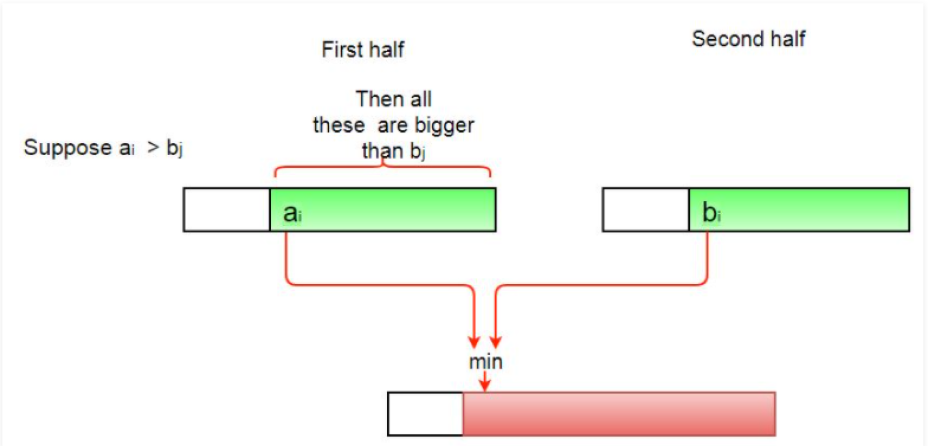
\includegraphics[width=0.85\textwidth]{mergeExplain.png}\\
    % \centerline{\includegraphics{process-explanation.png}}
    \tiny{Source - GeeksforGeeks}
    
    \label{explanation}
\end{figure}
\end{frame}

\begin{frame}{\textbf{Algorithm - Divide and Conquer}}
\textbf{For Cases 2 and 3}
\begin{itemize}
     \item Now for the second and the third case: If we encounter that situation, we again divide them up into further two arrays and repeat this recursively, until we have arrived on the base case - that includes just one element. And in this case, we know the inversions will be $0$, because there is just a single element in the array.
\end{itemize}

\begin{block}{Note}
Here, one more important thing is that in the first case, we require the arrays \textbf{L} and \textbf{R} to be sorted. So we need to incorporate that when we merge two arrays
\end{block}
\end{frame}

\section{Pseudo Code}
\begin{frame}{\textbf{Pseudo Code}}
\fontsize{8pt}{8}\selectfont
\begin{columns}

\begin{column}{0.5\textwidth}
\textbf{\underline{mergeTwoArrays}}\\
\vspace{3pt}
$i,k=beg$\\
  $j=end$\\
  $newarr$
\begin{algorithmic}
    \WHILE{$i< mid$ AND $j \le end$}
    \IF{$arr[i]<arr[j]$}
        \STATE newarr[k]=arr[i]
        \STATE increment k,i
    \ELSE
        \STATE newarr[k]=arr[j]
        \STATE invCount+= $mid-i$
        \STATE increment k,j
    \ENDIF
    \ENDWHILE
    
  \WHILE{$i<mid$}
    \STATE temp[k] = arr[i]
    \STATE increment k,i
  \ENDWHILE
  \WHILE{$j< end$}
    \STATE temp[k] = arr[j]
    \STATE increment k,j
  \ENDWHILE
  it = beg
  \WHILE{$it < end$}
    \STATE arr[it] = newarr[it]
    \STATE increment it
  \ENDWHILE
  \\return $invCount$
\end{algorithmic}
\end{column}

\begin{column}{0.5\textwidth}
\textbf{\underline{enhancedMergeSort}}\\
\vspace{3pt}
$\bm{arr}$: The Array\\
$\bm{beg}$: Start iterator\\
$\bm{end}$: End iterator\\
 $mid, invCount=0$
\begin{algorithmic}

  \IF{$end>beg$}
        \STATE mid = (beg+end)/2
        \STATE invCount += enhancedMergeSort(arr,left,mid)
        \STATE invCount += enhancedMergeSort(arr,mid+1,right)
        \STATE invCount += mergeTwoArrays(arr,left,mid+1,right)
    \ENDIF
    
    return $invCount$
\end{algorithmic}
\end{column}
\end{columns}
\end{frame}

\section{Time Complexity}
\begin{frame}{\textbf{Time Complexity}}
In the \textbf{Divide and Conquer} algorithm , the input array is divided into two halves each time it is processed.
As such it can be expressed with following recurrence relation,
\begin{center} T(n) = 2T(n/2) + $\theta$(n).\end{center}
    \textbf{O(N log(N))}
    \begin{figure}[htbp]
    % \center
     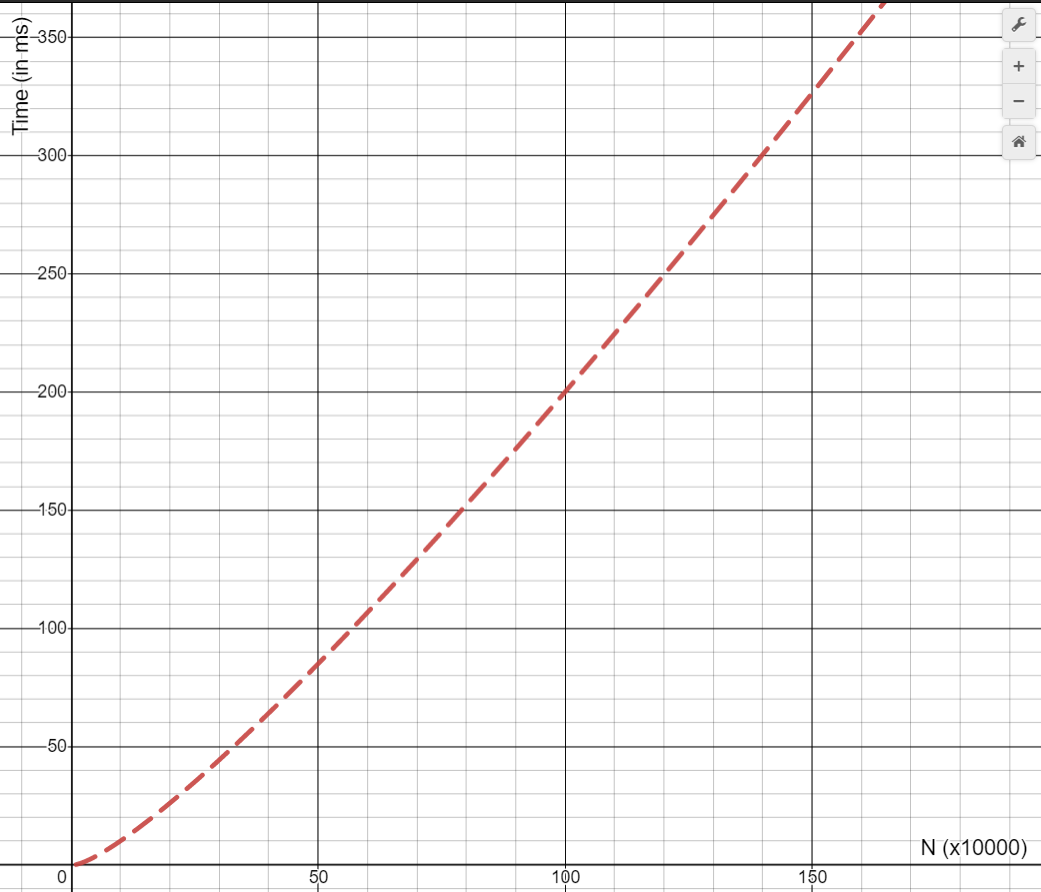
\includegraphics[width=0.55\textwidth]{timeComplexity.png}\\
\end{figure}
    
\end{frame}


\section{Space Complexity}
\begin{frame}{\textbf{Time Complexity}}
    \textbf{O(N)}
    \begin{figure}[htbp]
    % \center
     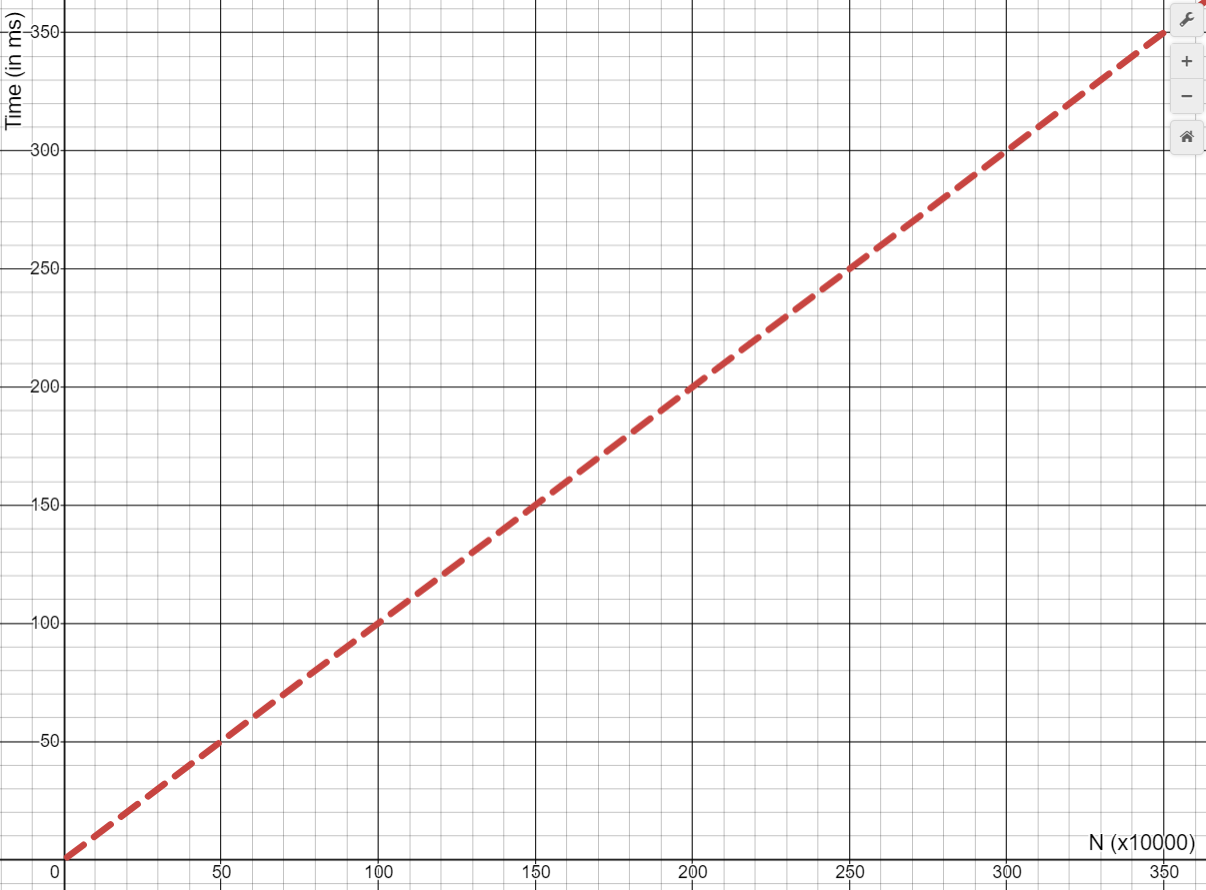
\includegraphics[width=0.85\textwidth]{spaceComplexity.png}\\
\end{figure}
    
\end{frame}


\section{References}
\begin{frame}{References}
\begin{thebibliography}{00}
\bibitem{b1}{Introduction to Algorithms by Thomas H. Cormen, Charles E. Leiserson, Ronald Rivest, Clifford Stein}\\
\bibitem{b2}{Introduction to Design and Analysis of Algorithms by Anany Levitin}\\
\bibitem{b3}{Algorithms by Robert Sedgewick and Kevin Wayne}
\end{thebibliography}
    
\end{frame}


\end{document}
